\chapter{Teoretická část}
%TODO write something nice

%%%%%%%%%%%%%%%%%%%%%%%%%%%%%%%%%%%%%%%%%%%%%%%%%
\section{Grafové databáze}

Grafy jsou velice přirozeným způsobem reprezentaci dat, zvláště v době, kdy většina dat je vytvářena uživateli v nestrukturované formě. Grafy pomocí uzlů a hran popisují objekty a vztahy mezi nimi s elegancí a přirozeností, jaké mohou jiné reprezentace dat těžko dosáhnout. Grafy usnadňují proces objevování informací v datech a přitom nevynucují náročné datové modelování skutečnosti do složitých datových struktur. Díky tomu, že grafy umožňují jednoduché prohladávání objektů, které mezi sebou mají vztahy (uzlů propojených hranami), jsou operace tohoto typu nad grafy relativně\footnote{Například vůči \nom{RDBMS}{relačním databázím} - čas nutný pro průchod přes několik hran je výrazně nižší než čas nutný ke spojení několika tabulek.} levné. 

\nom{GDB}{Grafové databáze} umožňují data reprezentovaná grafem ukládat a procházet tak, aby byly tyto přirozené výhody grafů zachovány a zároveň byly zajištěny alespoň některé vlastnosti \nom{RDBMS}{relačních databázových systémů}. 
% todo case studies https://neo4j.com/resources/top-use-cases-graph-databases-white-paper/

% TODO
% TODO cite 144 z holuba
\subsection{NoSQL}
\label{sec:gdb-nosql}
NoSQL databázové systémy sice nemají s touto prací mnoho společného, grafové databáze nicméně bývají zařazovány jako podkategorie NoSQL a bylo by tedy vhodné základní principe této skupiny technologií ve zkratce popsat. Samotná zkratka NoSQL je vykládaná různě, většinou jako \textit{"Not only SQL"\footnote{Eric Evans [82] Holubová TODO}} a vykládá se jako označení pro databáze nerelačního typu určené pro zpracování \textit{Big Data}\footnote{TODO definice big data, cite bp}. Mezi hlavní uváděné výhody NoSQL databází patří: 

\begin{itemize}
  \item{\textit{Škálovatelnost:}} Zatímco klasické databázové systémy využívají \textit{vertikální škálovatelnost}\footnote{TODO popis vetikální škálovatelnosti}, NoSQL databáze umožňují efektivní \textit{horizntální škálování}\footnote{TODO popis horizontálního škálování}. Data v NoSQL databázích bývají tedy typicky distribuovaná na několik uzlů\footnote{TODO vysvětlit clustery} a jejich zpracování tak může probíhat paralelně. 
  \item{\textit{Efektivní čtení:}} NoSQL datatabáze jsou silně orientovány na rychlé čtení (koncept \textit{write once, read many times}). Ve většině již nejsou data po zapsání do databáze nikdy modifikována, pouze nad nimi jsou vykonávány analýzy (dotazy). Za cenu potenciálně pomalejšího zápisu dat do databáze (který nám nevadí) získáme tedy výrazně vyšší rychlost čtení dat.  
  \item{\textit{Flexibilní datový model:}} NoSQL databáze buď nevyžadují žádné datové schéma, nebo je schéma volné (a lze ho tedy upravovat bez nutnosti úpravy stávajících dat). Dodržování schématu dat je tedy na aplikaci, která NoSQL databázi používá.  
  \item{\textit{Ekonomická stránka:}} jak již bylo uvedeno, relační databáze je nutné typicky škálovat vertikálně a to je nákladné\footnote{Jsou navyšovány prostředky jednoho stroje, což má technická omezení a čím více se těmto omezením blížíme, tím je škálování dražší. Vedlejším efektem této skutečnosti je často takzvaný \textit{vendor-locking}, tedy situace, kdy jsme nuceni používat specifický hardware (často od jedné konkrétní společnosti), který je velmi nákladný.}. Na druhé horizontální škálování je relativně levné - škáluje se přidáním nového uzlu. Vzhledem k tomu, že NoSQL databáze nevyžadují žádný konkrétní hardware, je možné používat takzvaný \textit{komoditní hardware} (uzly nemusí být hardwarově homogenní), který je levný.  
\end{itemize}

Aby těchto výhod NoSQL databáze dosáhly, využívají různé přístupy k reprezentaci dat a manipulaci s daty. Jejich hlavní rozdělení je následující: 

%TODO citace a příklady
\begin{itemize}
	% TODO cite redis
  \item{\textit{Databáze typu klíč-hodnota:}} Tyto databáze mají zcela volné datové schéma, jsou realizovány jako mapa klíčů a hodnot. Hodnota přitom typicků může nabývat několika datových typů (například číslo, text, binární řetězec, kolekce některého z předchozích). Operace nad tímto uložištěm jsou poměrně jednoduché a zpravidla neposkytují pokročilé nástroje pro analýzu dat na základě obsahu - pouze na základě klíče. 
  \item{\textit{Dokumentová databáze:}} Dokumentové databáze ukládají a spravují zpravidla strukturované dokumenty. Nejčastější formáty dokumentů jsou \nomExpl{\textit{JSON}\footnote{TODO popsat JSON}}{JavaScript Simple Object Notation} a \nomExpl{\textit{XML}\footnote{TODO popsat XML}}{Extensible Markup Language}. Narozdíl od databází typu klíč-hodnota umožňují dokumentové databáze přistupovat k dokumentům a analyzovat je dle jejich obsahu. 
  \item{\textit{Sloupcové databáze:}} Sloupcové databáze se skládají z tabulek, ve kterých může mít každý řádek libovolný počet sloupců (nezávislý na ostatních řádcích). Volné vkládání sloupců sloupců nijak nesnižuje výkon sloupcových databází, které bývají masivně distribuované.
  \item{\textit{Grafové databáze:}} Konečně posledním a pro nás nejzajímavějším typem NoSQL databází jsou grafové databáze. Tyto databáze jsou určené pro data, která je vhodné modelovat a dotazovat jako grafy (viz. kapitola \ref{sec:gdb-grafy}). Vnitřní reprezentace grafů může být různá podle toho, pro jaký typ grafových úlovh je daná databáze primárně určena.
\end{itemize}

% Typy NoSQL databází

\subsection{Grafy}
\label{sec:gdb-grafy}
% Matematická definice
Před popisem vlastních \nom{GDB}{grafových databází} blíže popíšeme grafy jako takové a jejich typy. Nejdříve uvedeme základní matematický rámec teorie grafů, se kterým budeme dále pracovat. 

Graf G je trojice (V, E, $\epsilon$), kde V je množina vrcholů\footnote{nebo také uzlů} a E množina hran. $\epsilon$ je přiřazení, které každé hraně přiřazuje: 
\begin{itemize} 
	\item{} množinu dvou vrcholů (koncové vrcholy) pro \textit{neorientovaný graf}
	\item{} uspořádanou dvojici vrzcholů (počáteční a koncový vrchol) pro \textit{orientovaný graf}
\end{itemize}

% Multigrafy / prosté grafy
Pokud graf neobsahuje paralelní hrany\footnote{nebo také multihrany}, tedy hrany, které mají stejné počáteční a koncové vrcholy (orientovaný graf), respektive stejné koncové vrcholy (neorientovaný graf), je označován jako \textit{prostý graf}. Naopak pokud graf paralelní hrany obsahuje, je označován jako \textit{multigraf}.\cite{Demlova17}

% Labeled grafy
Grafy z pohledu informačních technologií matematickou definici grafu dále rozšiřují. Umožňují definovat typy hran a uzlů, čímž vzniká \textit{ohodnocený graf}\footnote{Ohodnocený graf bývá také často označován jako labeled graf. Jeho opakem, tedy "neohodnoceným" grafem je jednovztahový nebo také homogenní graf.} Například ohodnocený graf na obrázku \ref{fig:labeled_graf} obsahuje dva typy uzlů (:OSOBA a :ČLÁNEK) a dva typy hran (:ZNÁ a :ČETL).

\begin{figure}
\begin{center}
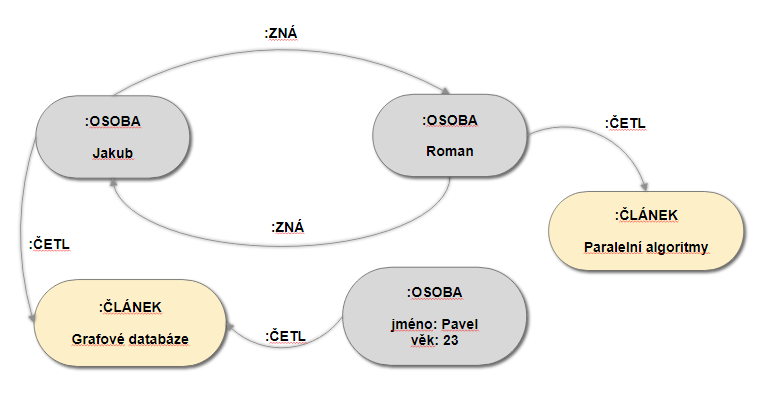
\includegraphics[width=14cm]{figures/labeled_graph}
\caption{Ohodnocený graf}
\label{fig:labeled_graf}
\end{center}
\end{figure}

% Property grafy
Ohodnocené grafy nám sice poskytují možnost rozlišit typy hran a uzlů, v mnoha situacích je ale žádoucí zachytit do grafu více informací. \textit{Atributové grafy} umožňují přiřadit hranám a uzlům libovolný počet atributů (dvojic klíč-hodnota), které obsahují informace o daném uzlu, respektive hraně. Příkladem může být věk osob, či datum vydání článku (viz obrázek \ref{fig:property_graf}). Většina grafových databází pracuje právě s atributovými grafy.\cite{Lal15}

\begin{figure}
\begin{center}
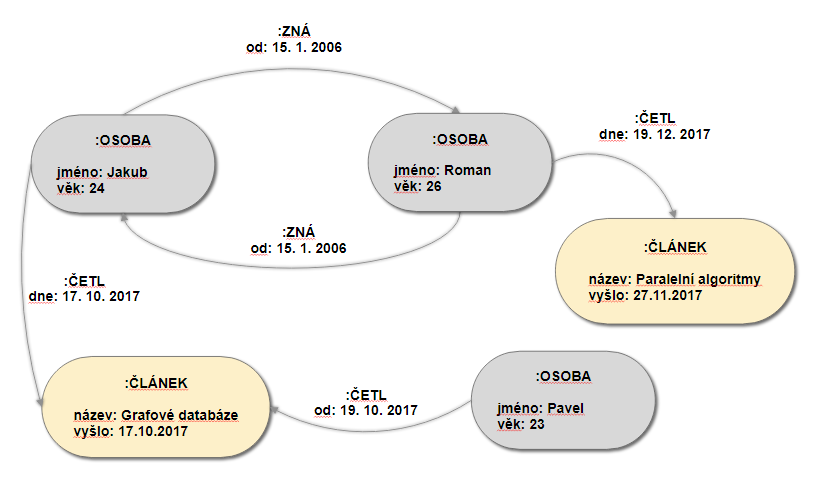
\includegraphics[width=14cm]{figures/property_graph}
\caption{Atributový graf}
\label{fig:property_graf}
\end{center}
\end{figure}

% Hypergrafy
Generalizací grafu je tzv. \textit{hypergraf}. Ten se proti grafu liší tím, že zatímco hrana grafu je množinou právě dvou vrcholů (či uspořádanou dvojicí v případě orientovaného grafu), hyperhrana (tedy hrana v hypergrafu) je mnoužinou jednoho a více vrcholů.\cite{Diestel00} Hypergrafy jsou používány k reprezentaci dat v mnoha oborech a některé GDB je přímo podporují (například HypergraphDB\footnote{http://hypergraphdb.org/}).


%TODO
\subsection{Perzistence}
Aby bylo možné v dalších kapitolách popsat pokročilé aspekty \nom{GDB}{grafových databází} (jako například indexování, či transakce), je nejdříve nutné popsat jejich základní principy. Nutnost ukládat data ve formě grafů je starší než pojem \nom{GDB}{grafové databáze} ve smyslu, v jakém je prezentován zde. Existuje tak mnoho způsobů uložení grafů z nichž ty nejběžnější zde popíšeme. Ještě předtím je nutno poznamenat, k jakým typům úkolů jsou \nom{GDB}{grafové databáze} zejména využívány. Častými grafovými úlohami jsou \nomExpl{BSF\footnote{Breadth-first search}}{průchod do hloubky} a \nomExpl{DFS\footnote{Depth-first search}}{průchod do šířky} a respektive jejich variace. Oba tyto algoritmy musí projít v nejhorším případě\footnote{Pro konkrétní problémy jsou často \nom{BFS} a \nom{DFS} algoritmy upravovány tak, aby bylo možné některé větve průchodu tzv. ořezávat - tedy procházet pouze jejich část, nebo je neprocházet vůbec.} všechny hrany grafu, je tedy vidět, že pro efektivitu \nom{GDB}{grafové databáze} je klíčová efektivity přechodu z jednodoho uzlu do (všech) jeho sousedů pomocí existujících hran.

% RDBMS (NEO Reasons to use graph databases)
% TODO zjistit zda se reálně někdy někde používalo a ozdrojovat
% TODO 166 holoubová
% https://inviqa.com/blog/graphs-database-sql-meets-social-network
Než se pustíme do popisu nativních grafových uložišť, krátce popíšeme možnost ukládání grafů pomocí \nom{RDBMS}{relačních databází}. Jedním z možných řešení může být dvojice tabulek \textit{UZLY} a \textit{HRANY}. Tabulka uzlů by obsahovala identifikátor uzlu a případné další parametry uzlu, tabulka hrany by obsahovala referenci na počáteční a koncový uzel hrany a případné další parametry hrany\footnote{V tomto případě předpokládáme orientovaný prostý atributový graf, pro jiné grafy by bylo nutné tuto strukturu upravit (což ale není těžké).}. Všechny hrany grafu je tedy možné získat pomocí spojení těchto tabulek pomocí cízího klíče, složitější průchody potom mohou být docíleny pomocí relace tabulky hran na sebe sama. Problém tohoto přístupu je právě zejména nutnost rekurzivních operací \textit{join} a jejich vysokých nákladů\footnote{Spojování tabulek pomocí cizích klíčů je jedna z nejdražších operací ve světě \nom{RDBMS}{relačních databází}}. Tyto problémy mohou být částečně eliminovány použitím sloupcových (TODO příklady) či dokumentových (todo příklady) NoSQL databází. Přestože v tomto případě nejsou používány rekurzivní join operace (ve světě NoSQL tato operace neexistuje), je k datům přistupováno pomocí prohledávání indexů a operace je tak stále výrazěn dražší, než při použití nativního grafového uložiště.\cite{Lal15} 
%TODO zmínit objektové db a objektovou reprezentaci grafu

%TODO všechna matematika jako italics

% Matice sousednosti
Nejzákladnější nativní reprezentací grafu je tzv. \textbf{matice sousednosti}. Ta využívá možnosti reprezentování hran grafu jako dvojice uzlů a reprezentuje graf jako matici \textit{M} o rozměrech \textit{|V|x|V|}, kde \textit{|V|} je počet uzlů grafu. Pokud existuje mezi uzly \textit{i} a \textit{j} hrana, pak bude \textit{M\textsubscript{i,j} != 0}. 
Pokud nás zajímá pouze existence hrany, nabývá matice pouze hodnot \textit{\{0, 1\}}. Pokud jsou hrany ohodnocené, pak nenulová hodnota buňky na dané pozici ukazuje nejen existenci hrany mezi danými uzly, ale také její ohodnocení. Pokud je graf neorientovaný, je matice symetrická. Pokud je graf orientovaný, potom \textit{M\textsubscript{i,j}} určuje existenci hrany z uzlu \textit{i} do uzlu \textit{j} a \textit{M\textsubscript{j,i}} naopak existenci hrany z uzlu \textit{j} do uzlu \textit{i}. 
Tato reprezentace grafu zajišťuje vysokou efektivitu přidávání, odstraňování a kontroly existence hran - tyto operace jsou okamžité, tedy $\Theta$(1).  Na druhou stranu přidání nového uzlu do grafu je nákladná operace, matice musí být přealokována a překopírována. Vzhledem k tomu, že paměťová náročnost matice sousednosti je kvadratická vzhledem k počtu uzlů a nezávisle na počtu hran (není tedy vhodná pro řídké matice\footnote{TODO poznámka o tom, že řídké matice jsou what u need}), je drahé i její překopírování - přidání nového uzlu má časovou složitost $\Theta$(|V|\textsuperscript{2}). 
Pro nalezení všech sousedních uzlů je nutné všechny uzly projít a zkontrolovat, zda hrana existuje, či nikoliv - $\Theta$(|V|). Hledání sousedních uzlů je nejčastější operací při průchodu grafu, tato reprezentace tedy není vhodná ani na složitější průchody. (TODO zdroje)

% Laplaceovská matice
Speciální variantou matice sousednosti je \textbf{Laplaceovská matice}. Ta má stejně jako matice sousednosti rozměry \textit{|V|x|V|}. Diagonála Laplaceovské matice ukazuje stupeň vrcholu a pokud existuje mezi dvěmi vrcholy hrana, je hodnota matice na dané pozici \textit{-1}. Pokud mezi vrcholy hrana naní, hodnota je \textit{0}. Hlavní výhodnou reprezentace grafu Laplaceovskou maticí je umožňění spektrální analýzy grafu\cite{Bernard93}, kdy jsou pomocí vlastních čísel matice analyzovány vlastnosti grafu.

% Matice incidence
Další možnou maticovou reprezentací grafu je \textbf{matice incidence}. Jedná se o dvoudimenzionální matici o rozměrech \textit{|V|x|E|}, kde každý sloupec matice odpovídá jedné hraně a řádek jednomu uzlu. Pokud je uzel \textit{v} účastníkem hrany \textit{e}, potom \textit{M\textsubscript{v,e} != 0}. Pokud se jedná o neorientované grafy, nabývá matice pouze hodnot \textit{\{0, 1\}}. Pokud je graf orientovaný, potom je odchozí hrana kódována jako \textit{-1} a příchozí jako \textit{1}. V případě ohodnoceného grafu mohou být hodnoty obecně všechna celá čísla (podobně jako u matice sousednosti), přičemž opět platí, že záporné číslo značí odchozí hranu a kládné číslo příchozí. Vzhledem k tomu, že pro většinu grafů platí, že počet hran |E| je vyšší než počet uzlů |V| (často, například u sociálních sítí, je výrazně vyšší), je tato reprezentace pro svou vysokou paměťovou náročnost ve většině případů nevhodná. Narozdíl od ostatních reprezentací ale umožňuje ukládání hypergrafů (hrany hypergrafu mohou zahrnovat libovolný počet vrcholů). Zatímco u běžného grafu by každý sloupec matice incidence obsahoval právě dva nenulové prvky, u hypergrafu jich může být libovolný počet. (TODO zdroje)

% List sousednosti 
Některé problémy matice sousednosti řeší \textbf{list sousednosti}. Ten je implementován jako množina listů, kde každému uzlu připadá jeden list sousedních uzlů (TODO viz obrázek). Paměťová náročnost této reprezentace je tedy $\Theta$(|V|+|E|), kde |V| je počet uzlů a tedy počet listů sousednosti a |E| je počet hran a tedy celkový počet prvků obsažených v listech sousednosti. List sousednosti je tedy výrazně úspornější reprezentace z paměťového hlediska, než je matice sousednosti a je tedy vhodný i pro řídké grafy. Zároveň umožňuje rychlé nalezení všech sousedních uzlů pro daný uzel, v listu jsou vypsány pouze ty uzly, se kterými je uzel propojen a procházení grafu je tak rychlé. Přidání hrany do grafu je přidáním jednoho prvku do listu (respektive dvou listů v případě neorientovaného grafu) a přidání uzlu je také relativně efektivní - znamená vytvoření nového listu a přidání ho do množiny ostatních listů. Drahé jsou naopak operace odebrání hrany (je nutné projít všechny sousedy obou koncových uzlů hrany) a odebrání uzlu (je nutné projít všechny hrany). Také ověření existence konkrétní hrany je relativně drahé (je potřeba opět projít všechny sousedy daného uzlu). Toto může být řešeno alternativní implementací, napříkald mohou být listy sousedů řazeny. Tím se sice sníží složitost ověření existence hrany, ale zvýší se složitost přidání nové hrany. (TODO zdroje)
Při reprezentaci velkých grafů pomocí listů sousednosti se používají kompresní techniky, díky kterým je možné dále snižovat paměťovou náročnost.\cite{Boldi04} % TODO možná více ke komprimovanému listu sousednosti

% TODO prostorová lokalita - 220 holub

% TODO RDF
% - (haxtree)
% - (bitmap)

% TODO obrázky

%TODO
\subsection{Typy dotazů}
%todo možná samostatná sekce?

\subsubsection{Traversal pattern}

Na rozdíl od indexově náročných množinových operací relačních databází využívají grafové databáze bezindexové místní prohledávání, tzv. traverzování.\cite{Anglels08} Relační databáze obsahují data typicky v normalizované formě v několika separátních tabulkách tak, aby bylo zamezeno duplikaci dat. Řádky těchto tabulek mohou být chápány jako objekty popsané svými vlastnostmi. Vztahy mezi objekty jsou definovány primárními a cizími klíči a musí být při dotazování explicitně vytvořeny spojením tabulek pomocí \textit{join} operace. Jak vyhledávání záznamů v tabulkách, tak spojování tabulek je (v ideálním případě) realizováno pomocí vyhledávacích indexů, které časovou složitost těchto operací značně snižují, obecně ale ne dostatečně. Databázové vyhledávací indexy jsou realizovány pomocí binárních vyhledávacích stromů (TODO cite), vyhledání zánamu má tedy složitost \textit{$\O$(n)}. 
Grafové databáze na druhé straně obsahují typicky pouze jednu strukturu - graf. Ten ve své fyzické reprezentaci obsahuje všechny hrany, které obsahuje, vztahy mezi objekty (vrcholy) v grafu jsou tedy implicitní, není potřeba je při každém dotazu vytvářet. Tato skutečnost s sebou nese výhody i nevýhody. 

%todo - nevýhoda - nedělitelnost grafu

%todo - výhoda - rychlost průchodů


%typy dotazů 
% - podgraf
% - nadgrafb


%TODO
\subsection{Indexy}
% - mining based 
% - non-mining base 

%TODO doplnit
\subsection{Transakce}

%ACID
Pojďme nejprve připomenout standardní transakční model světa relačních databází - \textbf{ACID}. Tento model říká, že transakce v databázovém systému musí být atomické (\textit{\textbf{A}tomocity}, tedy nedělitelné. Pokud tedy selže některá z operací transakce, selže celá transakce a je proved její \textit{rollback}\footnote{Rollback transakce je událost, která nastává, pokud transakce selže, nebo pokud je uživatelem explicitně vyvolána. Všechny kroky, které byly v rámci transakce provedeny jsou vráceny, po rollbacku transakce je tedy databáze ve stejném stavu, jako před spuštěním transakce. Opakem rollbacku je operace \textit{commit}, která potvrzuje všechny změny provedené v transakci.}. Nemůže se tedy stát, že by byla provedena jen část operací transakce a databáze se ocitla v nekonzistentním stavu. Jinými slovy, po provedení jakékoliv transakce (úspěšném i neúspěšném) bude databáze vždy konzistentní (\textit{\textbf{C}onsistency}). Všechny transakce jsou také izolované (\textit{\textbf{I}solated}), tedy transakce jsou na sobě navzájem nezávislé a neovlivňují si navzájem data. V případě, že dojde ke konfliktu několika transakcí, databázový systém konflikt vyřeší tak, aby byla tato vlastnost zachována\footnote{Existuje několik stuňu izolace transakcí , výčtem \textit{read uncommitted}, \textit{read committed}, \textit{repeatable read} a \textit{serializable}. Právě na úrovni izolace konfliktujících transakcí záleží, jakým způsobem bude konflikt vyřešen. Toto téma je podrobně rozebráno napříkald v TODO}. A konečně poslední vlastností transakcí v transakčním modelu ACID je trvanlivost (\textit{\textbf{D}urability}). Tato vlastnost zajistí, že změny provedené transakcí jsou trvalé. 

%BASE
Vlastnosti ACID transakčního modelu jsou klíčové pro relační databázové systémy, které mají širokou škálu využití. Pro svět NoSQL databází (do kterého bývají grafové databáze často řazeny) tento model ale není vhodný, a to především kvůli silnému důrazu na konzistenci dat a tedy jejich obtížné distribuovatelnosti\footnote{Distribuovanost dat je klíčová pro NoSQL databáze obecně, pro grafové databáze to ale ne vždy platí. Toto bude více rozebráno v kapitole \ref{sec:gdb-distribution}.}. Zaven je tedy alternativní transakční model - \textbf{BASE}. Ten říká, že systém numusí být nutně dostaupný vždy, stačí základní dostupnost (\textit{\textbf{B}asic \textbf{A}vailability}) - tedy dostupnost po většinu času. Mohou nastastat částečné výpadky, ale nikdy nedojde k výpadku celého systému\footnote{Tato vlastnost opět míří především na ty NoSQL databáze, které předpokládají vysokou distribuovanost dat a skládají se tedy z více uzlů. Od grafových databází, které distribuované nejsou očekáváme tedy dostupnost úplnou.}. Systém je v takzvaném volném stavu (\textit{\textbf{S}oft-state}), je dynamický, neustále docházi ke změnám. V případě distribuování a replikaci dat je důsledkem této vlastnosti mimo jiné to, že ne všechny repliky musí být nutně vzájemně konzistentní. A konečně, máme jistotu, že systém bude vždy "nakonec" uveden do konzistentního stavu (\textit{\textbf{E}ventual consistency}), ale nemusí být konzistentní v každém okamžiku. Například k vynucení konzistence může dojít až při čtení daty, při jejich zápisu nutná není\footnote{Jedná se o takzvanou \textit{lazy} konzistenci.}. Tento model tedy také umožňuje zachování jistoty konzistence dat, není ale automatická, jako tomu je u předchozího modelu.

Jak už bylo zmíněno, grafové databáze jsou typem NoSQL databází. Přesto většina grafových databází není NoSQL databází v pravém smyslu slova. Výsledkem tak je, že některé grafové databáze plně podporují ACID transakční model, jiné naopak BASE. Toto je blíže diskutováno v popisu konkrétních grafových databází (kapitola \ref{{sec:gdb-databaze}}). % TODO zdroje

% TODO
% https://link.springer.com/chapter/10.1007/978-3-319-29919-8_8

% TODO zámky

%TODO
\subsection{Distribuovatelnost}
\label{sec:gdb-distribution}
V kapitole \ref{sec:gdb-nosql} jsme zmínili, že distribuovanost dat je klíčovou vlastností NoSQL databází\footnote{Pokud je to možné, je vždy efektivnější když data distribuovaná nejsou. K jejich distribuování přikračujeme až ve chvíli, kdy nás k tomu nutí okolnosti - například velikost dat.}. Pro distribuci dat se využívá kombinování dvou technik - \textit{rozdělení (sharding)} a \textit{replikace} dat. 

% Sharding
Rozdělení dat je základním předpokladem pro jejich distribuci - musí dojít k rozdělení dat na vhodné množiny a ty uložit na různé uzly v clusteru. Při manipulaci s daty je tak přistopováno na jeden nebo více uzlů podle toho, jaká data jsou zpracovávána. Při rozdělování dat je bráno v potaz jejich rovnoměrné rozdělení, minimalizace počtu uzlů využívaných k provádění operací nad daty a optimalizace jejich fyzického rozmístění. 

% Replikace
Aby byla při případném výpadku části uzlů stále přístapná všechna data (všechny \textit{shardy}) jsou po částech mezi uzly několikrát replikována. Tím je zajištěno, že při selhání (ať už dočasném, nebo trvalém) jednoho uzlu nedojde ke ztrátě dat samotných, ani ke ztrátě přístupu k nim (pokud neselžou všechny repliky obsahující danou část dat). Počet, kolikrát jsou data v databázi replikována (replikační faktor) určuje mimo jiné algoritmus, pomocí kterého jsou data na repliky ukládána a rychlost jejich čtení. 

% Kontext grafů TODO
U grafových databází je ale distribuce dat (a tedy horizontální škálování) výrazně komplikovanější, než u ostatních NoSQL databází. Ty se typická skládají z několika struktur (tabulek, dokumentů, dvojic klíč-hodnota), zatímco obsahem grafové databáze je typicky pouze jediná struktura - graf. Rozdělení grafu na podgrafy je obtížný (zvláště pokud se jedná například o úplný graf), proto obecně ne mnoho grafových databází tuto možnost vůbec umožňuje. Přesto existují metody, které se distribucí grafu zabývají. Výsledná distribuce je potom typicky optimální pouze pro podmnožinu grafových úloh (distribucí grafu na několik uzlů se mění čas, v jakém je možné získat seznam sousedních vrcholů grafu v případech, kdy hrana mezi vrcholem a jeho sousedem spojuje dva podgrafy na dvou různých uzlech). 

%1D a 2D dělení matice sousednosti TODO




% strana 221 holub

%strana 9

% sharding str 30 vlevo dole


%Thus, it
% becomes difficult to scale graph databases beyond
% the confines of a single machine and at the same
% time, maintain the speed of a traversal across
% sharded borders. 

% However, at the expense of this
% drawback there is a significant advantage: there
% is a constant time cost for retrieving an adjacent
% vertex or edge. 


%TODO 
\subsection{Databáze - příklady}
\label{sec:gdb-databaze}

% TODO Neo4J

% TODO Sparksee

% TODO InfiniteGraph

% OrientDB

% Titan

% JanusGraph

% HyperGraph DB

% Jena

%TODO 
\subsection{Dotazovací jazyky}

% TODO nativní API

% TODO GraphQL

% TODO PQL

% TODO BPMN-Q

% TODO GOOD / GOQL

% TODO SPARQL (pro úplnost)
 
% TODO GREMLIN

% TODO Cypher


%%%%%%%%%%%%%%%%%%%%%%%%%%%%%%%%%%%%%%%%%%%%%%%%%
\section{Architektury a API} %todo maybe better heading
% https://cw.fel.cvut.cz/wiki/courses/a4m36aos/useful_materials

%todo RPC

%todo CORBA

%todo Java RMI

%todo mention HTTP 1.0 specification 1996

%todo mention XML specification 1996

%todo XML-RPC 
\subsection{XML-RPC}
V roce 1998 se objevil soubor pravidel, který popisuje jak využívat technilogie RPC, XML a HTTP k vzdálenému volání procedur přes internet - \nom{XML-RPC}{Remote Procedure Calling protokol používající XML pro komuniakci přes internet}.\cite{Winner99} XML poskytuje slovník pro popis RPC volání přenášená mezi počítači pomocí HTTP protokolu (ačkoliv je popsán také obecný přístup nezávislý na konkrétním protokolu). Uživatel pošle požadavek na server implementující protokol. Uživatelem je typicky software volající konkrétní proceduru vzdáleného systému. Volání může obasahovat více vstupních parametrů a očekává jedny výstupní hodnotu. Vstupní parametry mohou být vnořené do kolekcí jako jsou mapy a listy, mohou být tedy posílány rozsáhlé struktury. Proto je možné používat XML-RPC pro posílání objektů a struktur (jako vstupních i výsupních parametrů). Díky možnosti popsání předávaných informací pomocí XML umožňuje XML-RPC prakticky vytváření \nomExpl{API}{aplikačních rozhraní} a tím komunikaci dvou a více nehomogeních prostředí.\cite{Laurent01}  
% Because XML-RPC is layered on top of HTTP, it inherits the inefficiencies of HTTP. This
% does place some limitations on its use in large-scale, high-speed applications, but inefficiency
% isn't important in many places. Although there are definitely high-profile projects for which
% systems must scale to millions of transactions at a time, keeping response time to a minimum,
% there are also many projects to which systems need to send information or request
% processing far less often -- from once a second to once a week -- and for which response
% time isn't absolutely critical. For these cases, XML-RPC can simplify developers' lives
% tremendously. 

%todo SOAP, maybe UDDI and WSDL, maybe JAX-RPC
\subsection{SOAP}
Nástupcem XML-RPC se stal \nomExpl{SOAP}{Simple Object Access Protocol}. SOAP je postavený na podobných principech jako XML-RPC - používá XML jako formát zpráv a pro jejich přenos využívá protokolů aplikační vrstvy HTTP (standard), nebo SMTP. Cílem SOAPu je zajistit rozšířitelnost, neutralitu a nezávislost komunikace. Umožňuje komukaci procesů běžících na různých operačních systémech (pomocí XML) a volání webových služeb pomocí HTTP nezávisle na platformě a programovacím jazyku. 
Přestože specifikace SOAPu byla vytvořena už v roce 1998, byla zveřejněna až v roce 1999. Draft se nicméně nestal standardem \nomExpl{IETF}{Internet Engineering Task Force}\footnote{https://www.ietf.org/}.\cite{Box01} Až verze 1.2 se stala v roce 2007 doporučením \nomExpl{W3C}{World Wide Web Consortium}\footnote{https://www.w3.org/}.\cite{W3C07}
% https://en.wikipedia.org/wiki/SOAP
% https://www.w3.org/TR/2000/NOTE-SOAP-20000508/
% https://www.w3.org/TR/soap/

\nomExpl{WSDL}{Web Service Description Language} je formální strojově čitelný popis webové služby. Služba je popsána pomocí portů a koncových bodů


% The WSDL describes services as collections of network endpoints, or ports. The WSDL specification provides an XML format for documents for this purpose. The abstract definitions of ports and messages are separated from their concrete use or instance, allowing the reuse of these definitions. A port is defined by associating a network address with a reusable binding, and a collection of ports defines a service. Messages are abstract descriptions of the data being exchanged, and port types are abstract collections of supported operations. The concrete protocol and data format specifications for a particular port type constitutes a reusable binding, where the operations and messages are then bound to a concrete network protocol and message format. In this way, WSDL describes the public interface to the Web service.
% WSDL is often used in combination with SOAP and an XML Schema to provide Web services over the Internet. A client program connecting to a Web service can read the WSDL file to determine what operations are available on the server. Any special datatypes used are embedded in the WSDL file in the form of XML Schema. The client can then use SOAP to actually call one of the operations listed in the WSDL file using for example XML over HTTP.
% The current version of the specification is 2.0; version 1.1 has not been endorsed by the W3C but version 2.0 is a W3C recommendation.[1] WSDL 1.2 was renamed WSDL 2.0 because of its substantial differences from WSDL 1.1. By accepting binding to all the HTTP request methods (not only GET and POST as in version 1.1), the WSDL 2.0 specification offers better support for RESTful web services, and is much simpler to implement.[2][3] However support for this specification is still poor in software development kits for Web Services which often offer tools only for WSDL 1.1.[needs update][citation needed] For example, the version 2.0 of the Business Process Execution Language (BPEL) only supports WSDL 1.1.


%todo REST
% http://roy.gbiv.com/talks/200709_fielding_rest.pdf
% fielding disertation

%todo HATEOS

%%%%%%%%%%%%%%%%%%%%%%%%%%%%%%%%%%%%%%%%%%%%%%%%%
\section{Data Layer}

\section{Data(base) Layer Abstraction}
Abstrakce datové vrstvy (a databází) je historicky hojně diskutovaným tématem, %TODO zdroj
střetává se zde několik zájmů. Nejčastější argumenty proti tomuto principu míří na 
ztrátu výkonost při zařazování abstraktních vrstev. Tato ztráta výkonu je potom často způsobena 
právě úrovní abstrakce, konkrétně neschopností vývojáře použít konstrukty specifické pro dané databázové systémy. 
Je ale důležité si uvědomit, že odstranění vendor lockingu není jediným a ani primárním cílem \nom{DLA}{Database Layer Abstraction}.
Důležitějším cílem je zjednodušení aplikační logiky a její očištění o konstrukty z databázového světa. 

%TODO úrovně abstrakce viz http://blog.gauffin.org/2013/01/data-layer-the-right-way/ + dohledat lepší zdroj

%TODO data access alternatives - pokud to není to samé, ten samý zdroj

%TODO Data layer patterns -ten samý zdroj + https://thinkinginobjects.com/2012/08/26/dont-use-dao-use-repository/ or https://medium.com/@krzychukosobudzki/repository-design-pattern-bc490b256006 
% and https://martinfowler.com/eaaCatalog/repository.html (!)

%==================================%
%              NOTES               %
%==================================%

% - domain and data mapping layer